

\begin{frame}{XR System Architecture}
	\begin{columns}[t]
		\column{0.48\textwidth}
		\textbf{Hardware Components}
		
		\begin{itemize}
			\item Display devices: HMD, screens, AR glasses
			\item Tracking systems: SLAM, depth cameras, IMU
			\item Interaction devices: Controllers, haptic gloves, wearables
			\item Audio systems: Spatial audio
		\end{itemize}
		
		\column{0.48\textwidth}
		\textbf{Computing Infrastructure}
		
		\begin{itemize}
			\item Computing units: Standalone, PC-tethered, mobile
			\item Real-time processing: Graphics, physics, AI
			\item Sensor fusion: Multiple input modalities
			\item Feedback systems: Visual, auditory, haptic
		\end{itemize}
	\end{columns}
	
	\vspace{0.3cm}
	
	\begin{center}
		\small \textit{Integration of these components creates coherent, compelling, and safe interactive experiences}
	\end{center}
\end{frame}




\begin{frame}{Embodiment and Co-Presence}
	\textbf{\textcolor{gbAqua}{Embodiment}}: Perceiving a virtual body as one's own
	
	\begin{itemize}
		\item Reinforced by visuo-motor synchrony (virtual body mirrors real movements)
		\item Reinforced by visuo-tactile synchrony (virtual and physical touch align)
		\item Persists even with cognitive awareness of virtuality
	\end{itemize}
	
	\vspace{0.3cm}
	
	\textbf{\textcolor{gbAqua}{Co-Presence}}: In shared virtual environments
	
	\begin{itemize}
		\item Illusion of being spatially co-located with remote users
		\item Compresses social distance, enables natural interaction
		\item Important for collaborative and social XR scenarios
	\end{itemize}
	
	\citefooter{Botvinick \& Cohen, 1998; Gonzalez-Franco \& Lanier, 2017}
\end{frame}

\begin{frame}{Place Illusion and Plausibility Illusion}
	\textbf{\textcolor{gbAqua}{Two Complementary Illusions (Slater, 2009)}}
	
	\vspace{0.3cm}
	
	\begin{columns}[t]
		\column{0.48\textwidth}
		\textbf{Place Illusion (PI)}
		
		\begin{itemize}
			\item Feeling of occupying a real physical space
			\item ``Being there'' in the VE
			\item Grounded in immersion quality
		\end{itemize}
		
		\column{0.48\textwidth}
		\textbf{Plausibility Illusion (PSI)}
		
		\begin{itemize}
			\item Perceived credibility of events in the VE
			\item Sense that interactions genuinely happen
			\item Independent of ``being there'' feeling
		\end{itemize}
	\end{columns}
	
	\vspace{0.3cm}
	
	\textit{Both illusions together produce overall sense of presence}
	
	\citefooter{Slater, 2009}
\end{frame}

\begin{frame}{The Skarbez Taxonomy: A Multidimensional Design Space (Part 1)}
	\textbf{\textcolor{gbAqua}{Three Objective Dimensions}}
	
	\begin{columns}[t]
		\column{0.32\textwidth}
		\textbf{EWK}
		
		Environmental World Knowledge
		
		\small System's awareness of the real world (``what'' and ``where'')
		
		\column{0.32\textwidth}
		\textbf{IM}
		
		Immersion
		
		\small Quality and depth of visual, auditory, and haptic feedback
		
		\column{0.32\textwidth}
		\textbf{CO}
		
		Coherence
		
		\small Degree to which virtual objects behave consistently with user expectations
	\end{columns}
	
	\vspace{0.3cm}
	
	\textbf{\textcolor{gbAqua}{Key Insight}}
	
	These three objective dimensions give rise to distinct subjective experiences:
	\begin{itemize}
		\item \textbf{IM} alone → Place Illusion (PI)
		\item \textbf{CO} alone → Plausibility Illusion (PSI)
		\item \textbf{IM + CO} → Overall Presence (P)
		\item \textbf{All three} → Full Mixed Reality experience
	\end{itemize}
	
	\citefooter{Skarbez et al., 2021}
\end{frame}

\begin{frame}{The Skarbez Taxonomy: A Multidimensional Design Space (Part 2)}
	\begin{columns}[t]
		\column{0.48\textwidth}
		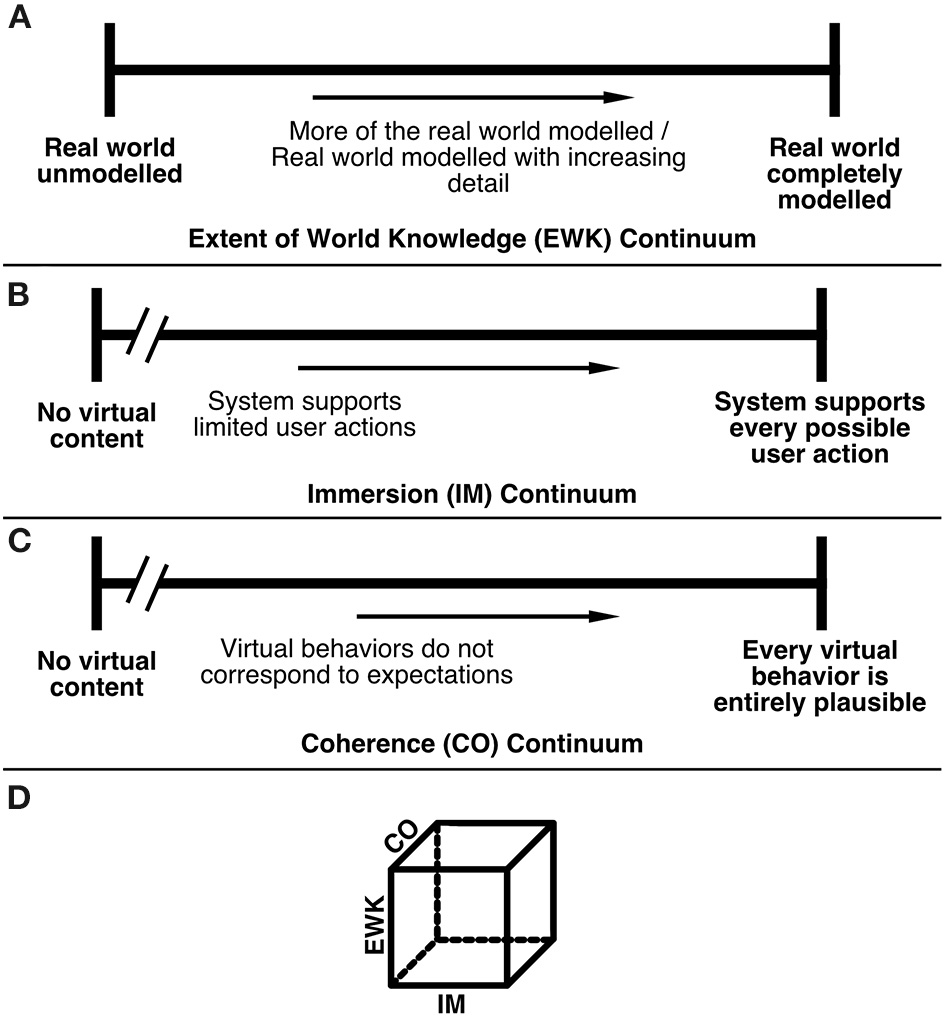
\includegraphics[width=\columnwidth]{figures/skarbez_fig5.png}
		
		\column{0.48\textwidth}
		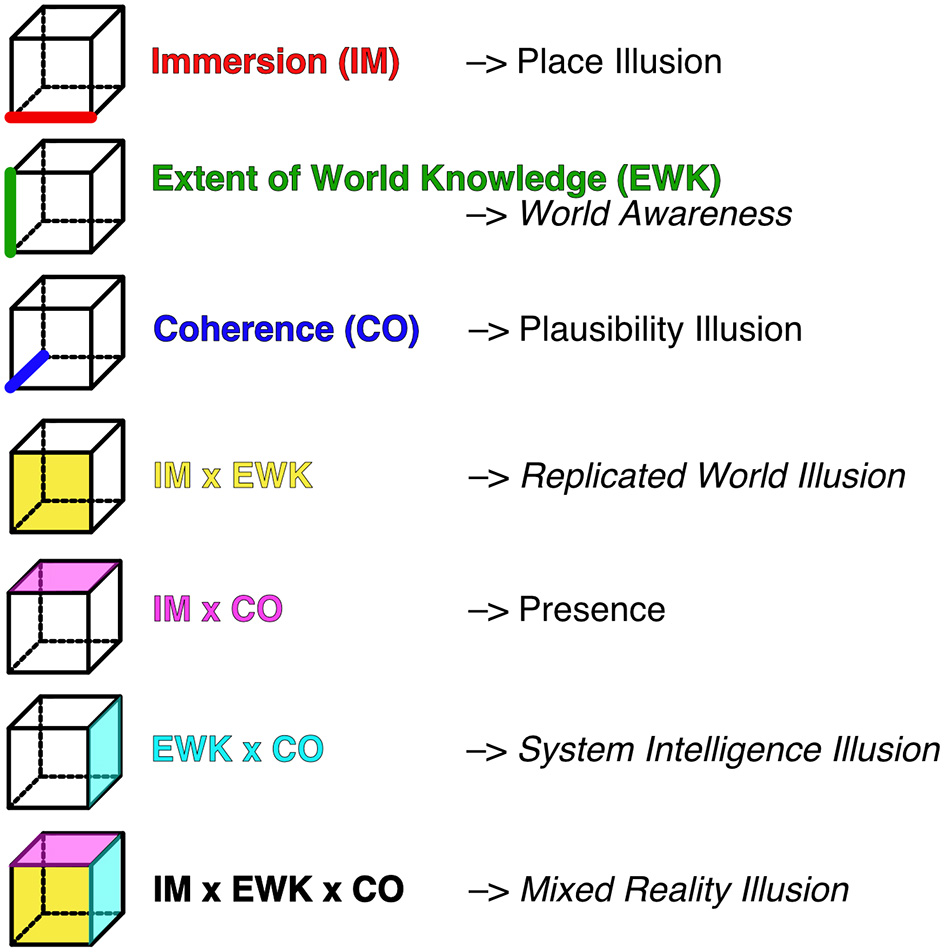
\includegraphics[width=\columnwidth]{figures/skarbez_fig6.png}
	\end{columns}
	
	\vspace{0.2cm}
	
	\small Design space for XR systems is multidimensional; choice between immersive and non-immersive carries theoretical consequences beyond hardware specifications.
	
	\citefooter{Skarbez et al., 2021}
\end{frame}